\subsection{Lokale Beleuchtungsmodelle}
\label{subsec:local_illumination_models}

Lokale Beleuchtungsmodelle aggregieren Daten lokal, also von
benachbarten Oberflächen. Diese Modelle sind in ihrem Umfang allerdings
limitiert, da sie normalerweise nur Lichtquellen sowie die Orientierung
einer Oberfläche einbeziehen. Sie ignorieren dabei aber die globale
Umgebung, in welcher sich eine Oberfläche befindet.  Die traditionell
verwendeten Algorithmen zur Berechnung der Sichtbarkeit von Oberflächen
verfügen über keine globalen Daten.\\
Das bekannteste lokale Beleuchtungsmodell ist das
\textit{Phong-Beleuchtungsmodell}, welches 1975 von Phong Bui-Tong
entwickelt wurde\parencite{phong_illumination_1975}. Es beschreibt
nicht-perfekte Reflektoren wie sie zum Beispiel ein
Apfel darstellt~\parencite[Kapitel 16, Seite 729]{foley_computer_1996}.

\begin{figure}[H]
    \centering
    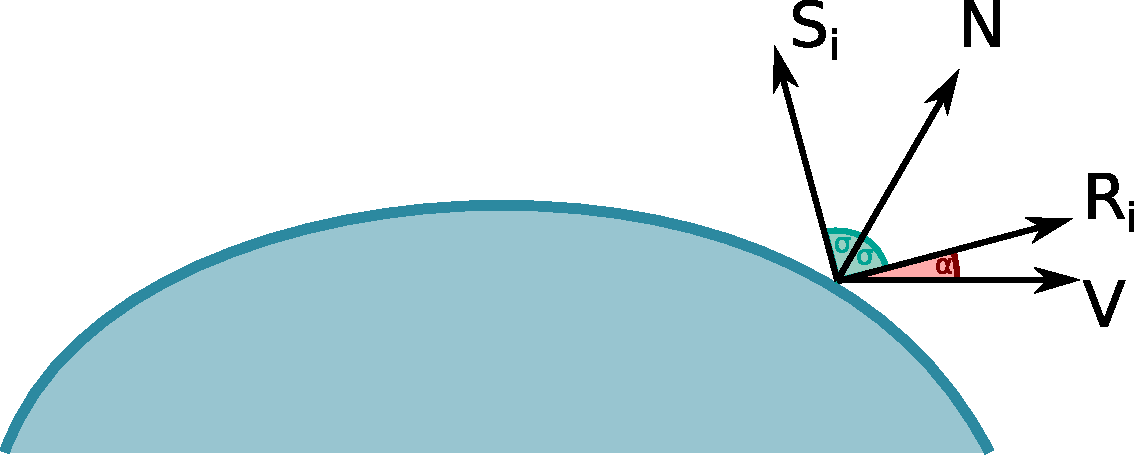
\includegraphics[width=0.6\textwidth]{img/phong_illumination_model.pdf}
    \caption{Illustration des Phong-Beleuchtungsmodelles\protect\footnotemark}\label{fig:phong_illustration}
\end{figure}
\footnotetext{Eigene Darstellung mittels Geogebra, angelehnt an~\cite{foley_computer_1996}[Kapitel 16, Seite 731, Abbildung 16.12]}

Das \textit{Phong-Beleuchtungsmodell} beschreibt die reflektierte
(Licht-) Intensität $I$ als Zusammensetzung aus der ambienten, der
diffusen und der ideal spiegelnden Reflexion einer Oberfläche:

\begin{gather}
    I = I_{\text{ambient}} + I_{\text{diffuse}} + I_{\text{specular}} + I_{\text{emissive}}
\end{gather}

Oder mathematisch ausgedrückt:

\begin{gather}\label{eq:phong_equation}
    I(\vv{V}) = k_{a} \cdot L_{a} +
                k_{d} \displaystyle\sum_{i=0}^{n - 1} L_{i} \cdot (\vv{S_{i}} \cdot \vv{N}) +
                k_{s} \displaystyle\sum_{i=0}^{n - 1} L_{i} \cdot {(\vv{R_{i}} \cdot \vv{V})}^{k_{e}}
\end{gather}

In der obigen Gleichung~\ref{eq:phong_equation} wurde der emissive Term
$I_{\text{emissive}}$ bewusst weggelassen, da er meistens für
Spezialeffekte statt für die Beleuchtung ``normaler'' Objekte benutzt
wird~\parencite{hughes_computer_2013}.

Wobei gilt:

\begin{itemize}
    \item $I(\vv{V})$\\
        Die reflektierte (Licht-) Intensität in Richtung des Vektors
        $\vv{V}$.

    \item $n$\\
        Anzahl Lichtquellen.

    \item $k_{a} \cdot L_{a}$\\
        Ambiente Komponente des Beleuchtungsmodelles. Mittels diesem
        Faktor wird versucht allem indirekten Licht der Szene gerecht zu
        werden. Bei $k_{a}$ handelt es sich um eine Konstante, welche
        den ambienten Anteils des Lichtes $L_{a}$ skaliert.

    \item $k_{d}$\\
        Konstante für die diffuse Komponente des reflektierten Lichtes,
        basierend auf der Wellenlänge bzw.\ der Frequenz.

    \item $\vv{S_{i}}$\\
        Richtung, in welcher das Licht der $i$-ten Lichtquelle ankommt,
        normalisierter Einheitsvektor.

    \item $\vv{N}$\\
        Einheitsnormale der Oberfläche.

    \item $k_{s}$\\
        Koeffizient der spiegelnden Komponente, basierend auf der
        Wellenlänge bzw. Frequenz.

    \item $\vv{R_{i}} = \vv{S_{i}} + 2(\vv{S_{i}} \cdot \vv{N})\vv{N}$\\
        Richtung, in welche das Licht der $i$-ten Lichtquelle
        reflektiert wird, normalisierter Einheitsvektor.

    \item $\vv{V}$\\
        Blickrichtung des Betrachters bzw.\ der Kamera.

    \item $k_{e}$\\
        Exponent, welcher von der Rauheit
        bzw.  Reflexion der Oberfläche abhängt.
    \item $L_{i}$\\
        Licht- bzw.\ Farbenintensität der $i$-ten Lichtquelle.
\end{itemize}

Der reflektive Vektor $\vv{R_{i}}$ ist gegeben durch

\begin{gather}
    \vv{R_{i}} = \vv{S_{i}} + 2(\vv{S_{i}} \cdot \vv{N})\vv{N}
\end{gather}

Damit die Energieerhaltung gewährleistet ist, muss weiter $k_{d} + k_{s}
< 1$ gelten. Der Winkel zwischen $\vv{R}$ und $\vv{V}$ wird mittels
$\cos(\alpha)$ ermittelt.
